%
% main.tex -- Paper zum Thema meteor
%
% (c) 2019 Hochschule Rapperswil
%
\chapter{Analyse von Meteor-Echos\label{chapter:meteor}}
\lhead{Analyse von Meteor-Echos}
\begin{refsection}
\chapterauthor{Dominic Hüppi}

Seit dem Beginn des Menschen blickt dieser dem Himmel entgegen.
Bereits in der Steinzeit, der frühesten Epoche der Menschheitsgeschichte, nahm die Beobachtung von Sonne und Gestirn ihre Anfänge.
Neben der Sonne und dem Mond wirkten Meteore oder umgangssprachlich 'Sternschnuppen' dabei schon immer eine Faszination auf ihre Beobachter aus.
In der Antike galten sie als Vorzeichen für den Tod, im frühen Christentum waren sie ein Zeichen der Seelenerlösung und im Mittelalter überbrachten sie angeblich die Mahnungen Gottes.

Heutzutage, in Zeiten der modernen Astronomie, schauen wir den herabstürzenden Leuchterscheinungen etwas entspannter und objektiver (ausgenommen sind die Flacherdler) entgegen.
Wenn wir heute eine `Sternschnuppe' beobachten gehen einem die Wünsche in Erfüllung, aber bloss keinem seinen Wunsch verraten.
Für Astronomen gelten Meteore als wichtige Zeugen aus der Frühzeit des Sonnensystems und für den heute ungemein wichtigen `Influencer' bilden sie ideale Sujets für den nächsten Auftritt in den sozialen Medien.
Und wer hat schon nicht fasziniert dem Himmelgestirn entgegengeblickt und den aufleuchtenden Lichtstrahl romantisiert.

Meteore zeigen sich als überaus interessantes Ereignis.
Das folgende Kapitel bringt weitere Einblicke in die Welt der Meteore und welche Rolle `Wavelets' darin einnehmen.
\begin{figure}
	\centering
	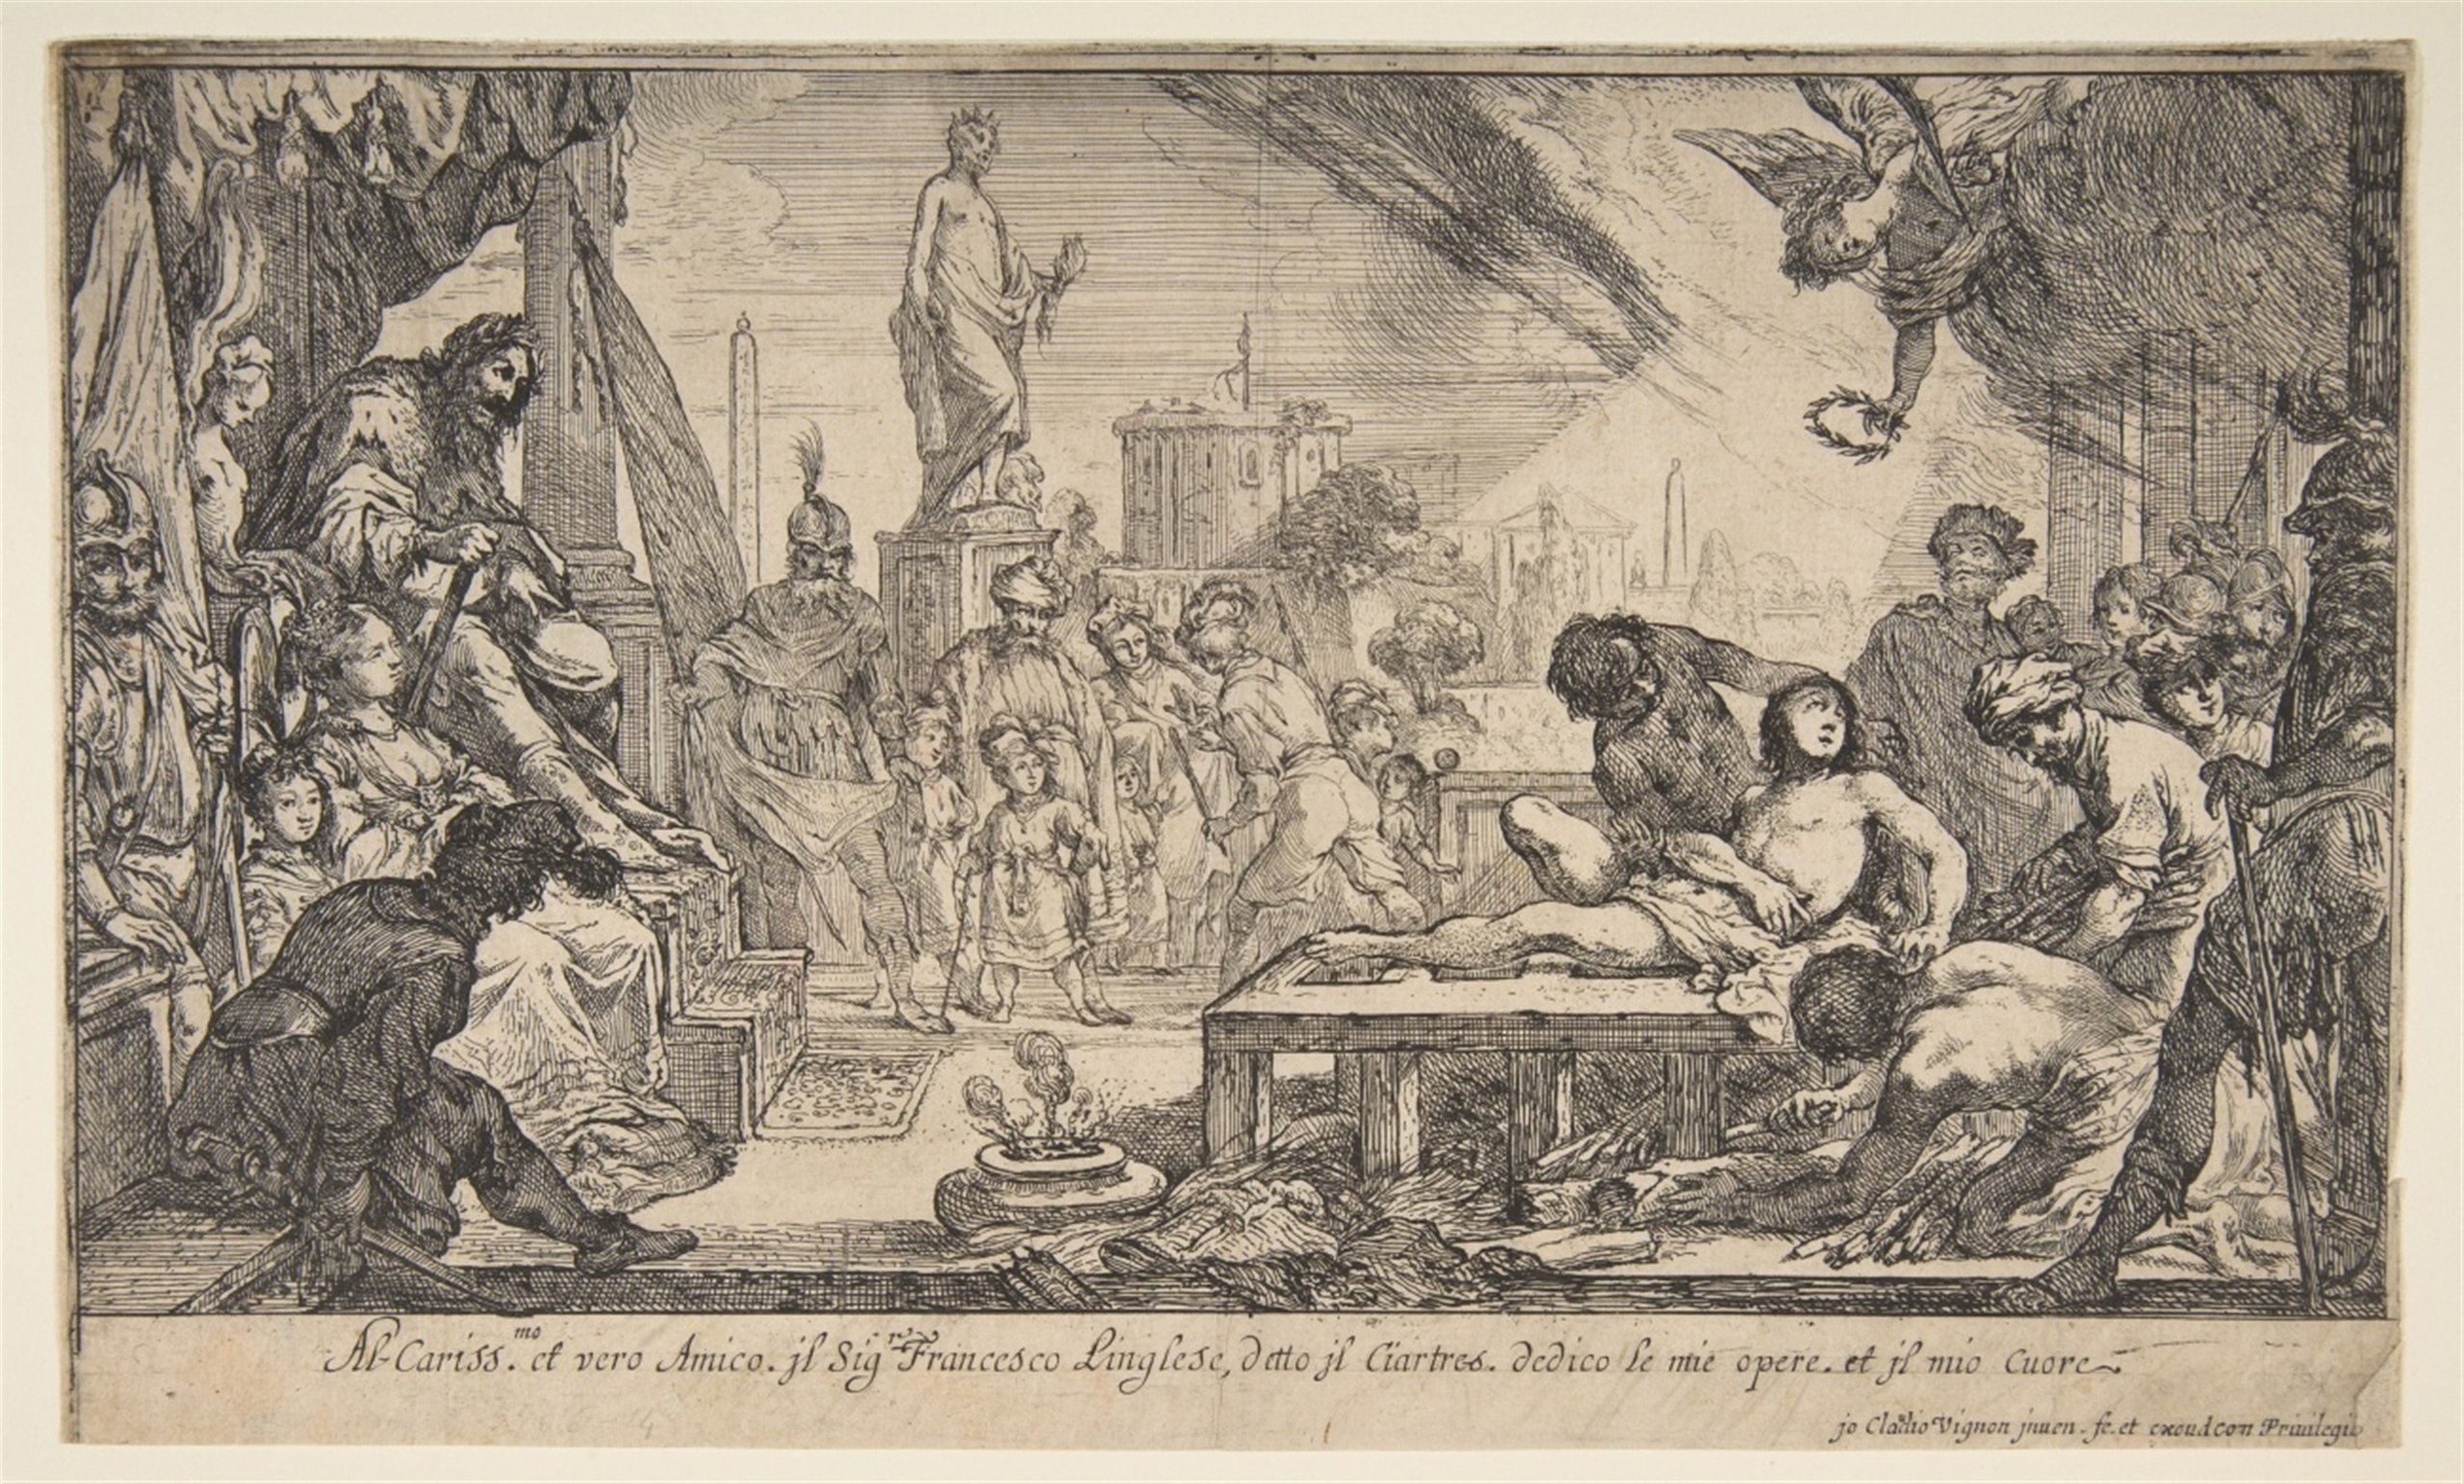
\includegraphics[width=0.7\linewidth]{papers/meteor/images/claudeVignonMartyriumDesHeiligenLaurentius}
	\caption{Martyrium des heiligen Laurentius von Rom im Jahr 258. 
		Hinrichtung auf glühendem Eisenrost, da er sich weigerte den Kirchenschatz dem Kaiser auszuhändigen.\cite{buch:joeckle}
		In der darauffolgenden Nacht trat ein starker Sternschnuppenregen auf, bekannt als Laurentiustränen oder Perseiden. 
		Dieser Meteorstrom ist alljährlich wiederkehrend und kann in der ersten Augusthälfte beobachtet werden.\cite{gemaelde:vignon}}
	\label{fig:claudevignonmartyriumdesheiligenlaurentius}
\end{figure}

\section{Meteore}
\rhead{Abschnitt}

Der Begriff Meteor hat sich über die Zeit verändert. 
Bis zum vorherigen Jahrhundert, wurden sämtliche vom Himmel fallende Objekte Meteore genannt. 
Auch Regen, Schnee oder Hagel gehörten dazu. 
Diese Bedeutung des Wortes Meteor ist bis heute in der Wetterkunde als Meteorologie beständig geblieben.
Allgemein bezeichnet man heute nur noch kleine Objekte, welche beim Eindringen in die Erdatmosphäre eine Lichtaussendung hervorrufen, als Meteore.  
Die Erde ist zur jederzeit einem Bombardement aus unzähligen Kleinkörper aus dem All ausgesetzt. 
Diese erhitzen sich durch Reibung an den Luftschichten sehr stark und verglühen in der Atmosphäre. 
Die Kleinkörper sind of nur wenige Kubikmillimeter gross und werden in die leuchtschwachen `Sternschnuppen' und die leuchtstarken `Feuerkugeln' unterteilt.
Grössere Objekte, welche die Lichterscheinung einer Feuerkugel hervorrufen, jedoch nicht vollständig in der Atmosphäre verglühen und auf die Erdoberfläche treffen, werden als `Meteorite' bezeichnet.

Entgegen der allgemeinen Annahme, Meteore stürzen wegen der Anziehungskraft der Erde auf sie nieder, ist es viel mehr eine Kollision zweier sich unabhängig bewegender Himmelskörper. 
Die Flugbahn des Meteors wird dabei nur sehr geringfügig durch das Gravitationsfeld der Erde beeinflusst.
Aufgrund der Bahnform ist man heute der Meinung die Objekte ihrer kosmischen Herkunft zuordnen zu können. 
Zwei dieser Herkünfte sind besonders interessant und erklären zudem die Tatsache, dass Meteore oft nicht als Einzelerscheinung auftreten. 
Meteore mit Ellipsen kurzer Umlaufzeit entstammen Planeten oder kleineren Objekten unseres Sonnensystems und werden Planetarische Meteore genannt.
Kometarische Meteore hingegen sind die Begleiterscheinungen eines Kometen. 
Kometen sind im Gegensatz zu Meteoren grosse Himmelskörper mit einem Durchmesser von einigen Kilometern.
Auf ihrer Bahn durchs Sonnensystem ziehen sie einen durch Ausgasen erzeugten leuchtenden Schweif hinter sich her.
Dieser Schweif besteht aus vielen kleinen Objekten, welche sich vom Kometen abscheiden und als kometarische Meteore fortbestehen.
Deshalb ist es nicht verwunderlich, dass gewisse Meteorschauer, wie zum Beispiel der erwähnte Perseiden, zyklisch auftreten.\cite{lexikon:meyer}

Meteore treten mit 30 bis 70 Kilometern pro Sekunde in die Erdatmosphäre ein. 
Die im Durchmesser nur wenige Millimeter grossen Objekte werden aufgrund der grösser werdenden Dichte der Luftschicht Reibung ausgesetzt.
Die auftretenden Kräfte erhitzen den Meteor so stark, dass dieser abdampfendes Material hinterlässt.
Dies erzeugt hinter dem herabstürzenden Objekt eine Plasmaspur, welche zusammen mit den Luftatomen eine Rekombination verursacht.
Die Rekombination stellt die Umkehrung der Ionisierung dar. 
Dabei werden elektrisch positiv und elektrisch negativ geladenen Teilchen vereint.
Die bei diesem Prozess entstehende Energie wird durch die Emission von Photonen abgegeben, was zu einer Leuchterscheinung führt.\cite{web:brodbeck}


\section{Detektieren von Meteoren}
\rhead{Abschnitt}

Es ist möglich Meteore mit optischen Systemen zu erfassen. 
Da diese Ereignisse nur kurze Transienten haben gestaltet sich dies als schwierig.
Ebenso ist die Beobachtung stark von den Wetterbedingungen sowie den Lichtverhältnissen abhängig.
Mittels Radio-Echo wird eine kontinuierliche Meteorbeobachtung erreicht. 

\section{Auswertung der Radio-Signale}
\rhead{Abschnitt}

\section{Schlussfolgerung}
\rhead{Schlussfolgerung}

\printbibliography[heading=subbibliography]
\end{refsection}
